% Upper bounds for the exponent omega of matrix multiplication, 1969-2024 (step plot).
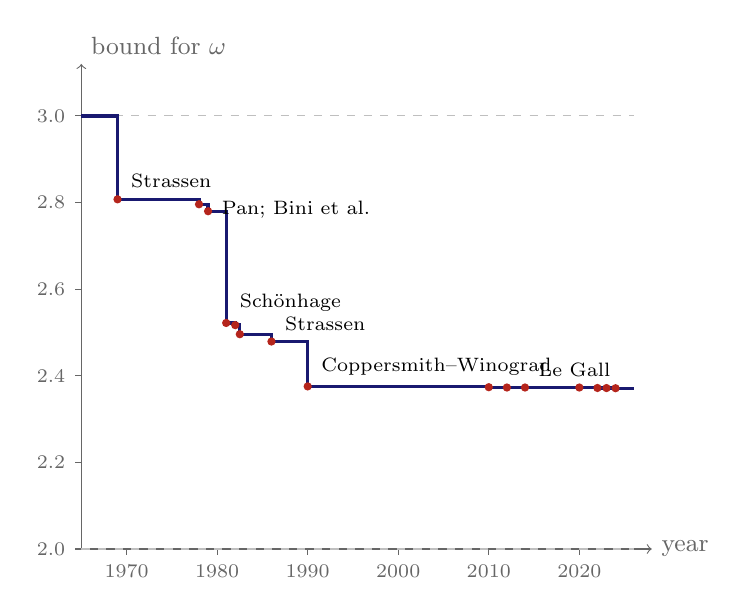
\begin{tikzpicture}[font=\small]
\draw[->,black!60] (0,0) -- (7.245,0) node[right] {year};
\draw[->,black!60] (0,0) -- (0,6.160) node[above right] {bound for $\omega$};
\draw[black!60] (0.575,0) -- ++(0,-0.08) node[below,font=\scriptsize] {1970};
\draw[black!60] (1.725,0) -- ++(0,-0.08) node[below,font=\scriptsize] {1980};
\draw[black!60] (2.875,0) -- ++(0,-0.08) node[below,font=\scriptsize] {1990};
\draw[black!60] (4.025,0) -- ++(0,-0.08) node[below,font=\scriptsize] {2000};
\draw[black!60] (5.175,0) -- ++(0,-0.08) node[below,font=\scriptsize] {2010};
\draw[black!60] (6.325,0) -- ++(0,-0.08) node[below,font=\scriptsize] {2020};
\draw[black!60] (0,0.000) -- ++(-0.08,0) node[left,font=\scriptsize] {2.0};
\draw[black!60] (0,1.100) -- ++(-0.08,0) node[left,font=\scriptsize] {2.2};
\draw[black!60] (0,2.200) -- ++(-0.08,0) node[left,font=\scriptsize] {2.4};
\draw[black!60] (0,3.300) -- ++(-0.08,0) node[left,font=\scriptsize] {2.6};
\draw[black!60] (0,4.400) -- ++(-0.08,0) node[left,font=\scriptsize] {2.8};
\draw[black!60] (0,5.500) -- ++(-0.08,0) node[left,font=\scriptsize] {3.0};
\draw[black!25,dashed] (0,5.500) -- (7.015,5.500);
\draw[black!25,dashed] (0,0.000) -- (7.015,0.000);
\draw[MidnightBlue,very thick] (0.000,5.500) -- (0.460,5.500) -- (0.460,4.441) -- (1.495,4.441) -- (1.495,4.378) -- (1.610,4.378) -- (1.610,4.290) -- (1.840,4.290) -- (1.840,2.871) -- (1.955,2.871) -- (1.955,2.843) -- (2.013,2.843) -- (2.013,2.728) -- (2.415,2.728) -- (2.415,2.635) -- (2.875,2.635) -- (2.875,2.065) -- (5.175,2.065) -- (5.175,2.055) -- (5.405,2.055) -- (5.405,2.051) -- (5.635,2.051) -- (5.635,2.051) -- (6.325,2.051) -- (6.325,2.051) -- (6.555,2.051) -- (6.555,2.045) -- (6.670,2.045) -- (6.670,2.044) -- (6.785,2.044) -- (6.785,2.042) -- (7.015,2.042) -- (7.015,2.042);
\fill[BrickRed] (0.460,4.441) circle (1.5pt);
\node[font=\scriptsize,anchor=south west] at (0.510,4.461) {Strassen};
\fill[BrickRed] (1.495,4.378) circle (1.5pt);
\fill[BrickRed] (1.610,4.290) circle (1.5pt);
\node[font=\scriptsize,anchor=west] at (1.660,4.310) {Pan; Bini et al.};
\fill[BrickRed] (1.840,2.871) circle (1.5pt);
\node[font=\scriptsize,anchor=south west] at (1.890,2.891) {Sch\"onhage};
\fill[BrickRed] (1.955,2.843) circle (1.5pt);
\fill[BrickRed] (2.013,2.728) circle (1.5pt);
\fill[BrickRed] (2.415,2.635) circle (1.5pt);
\node[font=\scriptsize,anchor=south west] at (2.465,2.655) {Strassen};
\fill[BrickRed] (2.875,2.065) circle (1.5pt);
\node[font=\scriptsize,anchor=south west] at (2.925,2.085) {Coppersmith--Winograd};
\fill[BrickRed] (5.175,2.055) circle (1.5pt);
\fill[BrickRed] (5.405,2.051) circle (1.5pt);
\fill[BrickRed] (5.635,2.051) circle (1.5pt);
\node[font=\scriptsize,anchor=south west] at (5.685,2.071) {Le Gall};
\fill[BrickRed] (6.325,2.051) circle (1.5pt);
\fill[BrickRed] (6.555,2.045) circle (1.5pt);
\fill[BrickRed] (6.670,2.044) circle (1.5pt);
\fill[BrickRed] (6.785,2.042) circle (1.5pt);
\end{tikzpicture}
